\documentclass[]{article}
\usepackage[T1]{fontenc}

\usepackage{graphicx}
\usepackage{parskip}
\usepackage[]{hyperref}
\usepackage[french]{babel}
\usepackage{subcaption}

\author{Erwan LEMATTRE, Yannis CHUPIN}
\title{Rapport mi-projet\\Fairness pour l'IA}

\begin{document}
    \maketitle
    \newpage
    \tableofcontents
    \newpage

    \section{Introduction}
    Ce projet a pour objectif d'analyser les accidents de la circulation routière afin de pouvoir dire 
    à partir des données d'un véhicule accidenté si l'accident est mortel ou non.
    Les données sont des données libres mises à disposition par le \textit{Ministère de l'intérieur et des 
    Outre-Mer}. Le jeu de donnée correspond aux accidents de 2005 à 2022 en France. Nous allons dans une première 
    partie analyser ces données afin d'extraire les informations utiles à l'apprentissage et de pouvoir repérer 
    d'éventuelles sources de biais pour notre modèle.
    
    Vous pouvez retrouver le code sur le GitHub du projet. Le fichier \texttt{main.ipynb} contient 
    le code principale que nous allons suivre tout au long de ce rapport. Le fichier \texttt{utils.py} 
    contient toutes les fonctions auxilières que nous utilisons dans le fichier principale.

    \section{Découverte du jeu de données}
    \subsection{La base de données}
    La base de données est composée de plusieurs tables: \textit{usagers}, \textit{vehicules}, \textit{lieux} et 
    \textit{caracteristiques}. Nous avons joint ces quatres parties pour obtenir un dataframe contenant une 
    cinquantaine de colonnes. 
    Ci-dessous une rapide présentation des différentes données disponibles.

    \begin{center}
        \begin{tabular}{ |c|p{9cm}| }
            \hline
            \textbf{Attribut} & \textbf{Description} \\
            \hline
            \textit{Num\_Acc} & Numéro d'identifiant de l'accident \\
            \textit{jour mois} & Jour de l'accident, mois de l'accident \\
            \textit{an} & Année de l'accident. \\
            \textit{hrmn} & Heure et minutes de l'accident. \\
            \textit{lum} & Lumière: conditions d'éclairage dans lesquelles l'accident s'est produit. \\
            \textit{dep} & Département: Code INSEE.\\
            \textit{com} & Commune: Le numéro de commune est un code donné par l‘INSEE. \\
            \textit{agg} & Localisation dans une aglomération ou non. \\
            \textit{int} & Si intersection: type d'intersection. \\
            \textit{atm} & Conditions atmosphériques. \\
            \textit{col} & Type de collision. \\
            \textit{adr} & Adresse postale: variable renseignée pour les accidents survenus en agglomération. \\
            \textit{lat} & Latitude. \\
            \textit{long} & Longitude. \\
            \textit{catr} & Catégorie de route (type de route). \\  
            \textit{voie} & Numéro de la route. \\  
            \textit{circ} & Régime de circulation. \\  
            \textit{nbv} & Nombre total de voies de circulation. \\  
            \textit{vosp} & Signale l'existence d'une voie réservée. \\  
            \textit{prof} & Profil en long décrit la déclivité de la route à l'endroit de l'accident. \\  
            \textit{plan} & Tracé en plan de la route. \\  
            \textit{surf} & Etat de la surface de la route. \\  
            \textit{infra} & Aménagement --- Infrastructure s'il y en a. \\  
            \textit{situ} & Situation géographique de l'accident. \\  
            \textit{vma} & Numéro d'identifiant de l'accident. \\
            \textit{id\_vehicule} & Identifiant du véhicule, foreign key. \\
            \textit{catv} & Catégorie du véhicule accidentée. \\  
            \textit{obs} & Type d'obstacle heurté. \\
            \textit{obsm} & Type d'obstacle mobile heurté. \\
            \textit{choc} & Point de choc initial. \\
            \textit{manv} & Manoeuvre principale avant l'accident. \\
            \textit{catu} & Catégorie d'usager (Conducteur, passager, piéton) \\
            \textit{grav} & Gravité de l'accident pour l'usager. \\
            \textit{sexe} & Sexe du conducteur de la voiture (calculé dans le notebook). \\
            \textit{trajet} & Motif du déplacement au moment de l'accident. \\
            \textit{mortal} & Insique si le véhicule est impliqué dans un accident mortel. Attribut calculé dans le notebook. \\
            \hline
        \end{tabular}
    \end{center}

    \subsection{Répartition des données}
    Afin de pouvoir conserver les données utiles pour l'apprentissage nous avons analysé la répartition des 
    différentes données dans notre dataframe.
    Nous avons ainsi pu faire différentes observations. 
    \\
    Voici quelques-unes d'entre elles qui nous sont ensuite
    utiles pour la préparation des données.
    \subsubsection{Catégories de véhicule}
    La base de données nous donne beaucoup de catégories différentes. Nous avons cependant pu remarquer 
    que la majorité des véhicules sont dans seulement 5 catégories.
    \begin{figure}[ht]
        \centering
        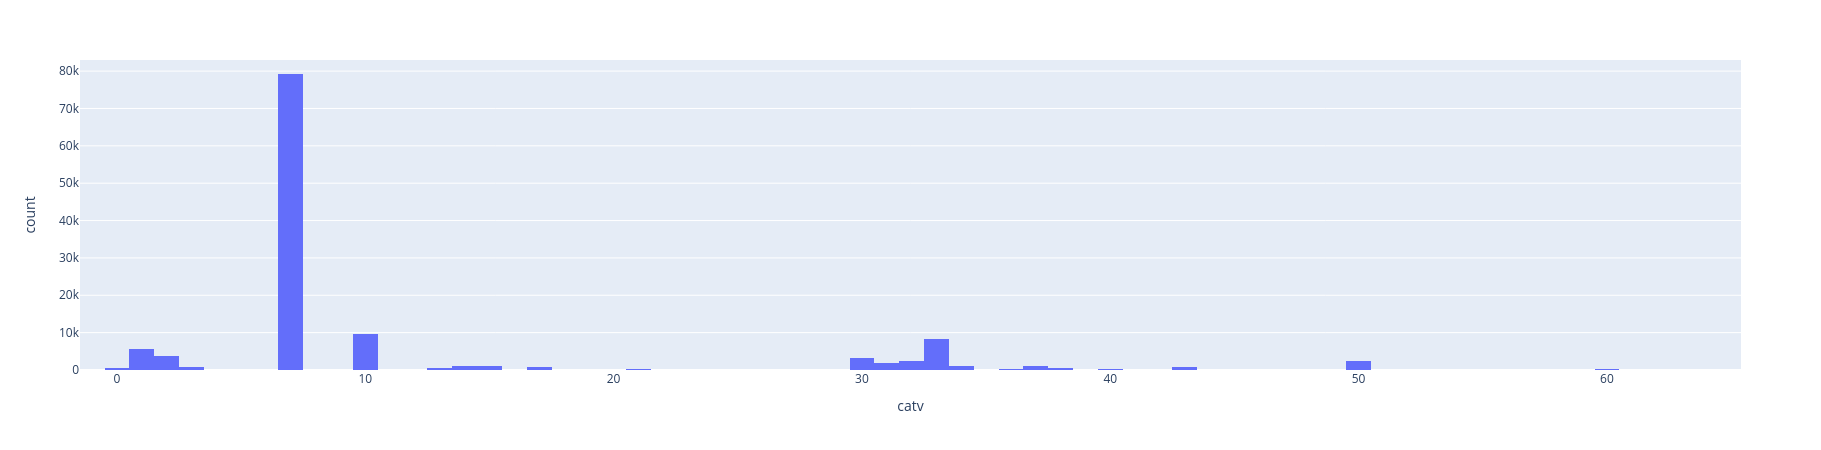
\includegraphics[width=12cm]{./img/catv1.png}
        \caption{Répartition des catégories de véhicules}
    \end{figure}

    \subsubsection{Gravité de l'accident}
    En affichant l'effectif d'accidents mortels nous avons pu remarquer qu'ils ne représentent qu'une 
    infime partie des accidents. Le peu de données sur ces accidents ne nous permet pas l'apprentissage 
    d'un modèle. C'est la raison pour laquelle nous avons décidé de nous intéresser non pas à la mortalité 
    à l'échelle d'une personne mais plutôt à l'échelle d'un accident. Nous nous mettons pour cela au niveau d'un 
    véhiule car cela nous permet de conserver plus d'informations (à l'échelle d'un accident on aurait 
    dû enlever trop d'informations pour conserver seulement les attributs plus généraux à l'accident).

    \begin{figure}[ht]
        \centering
        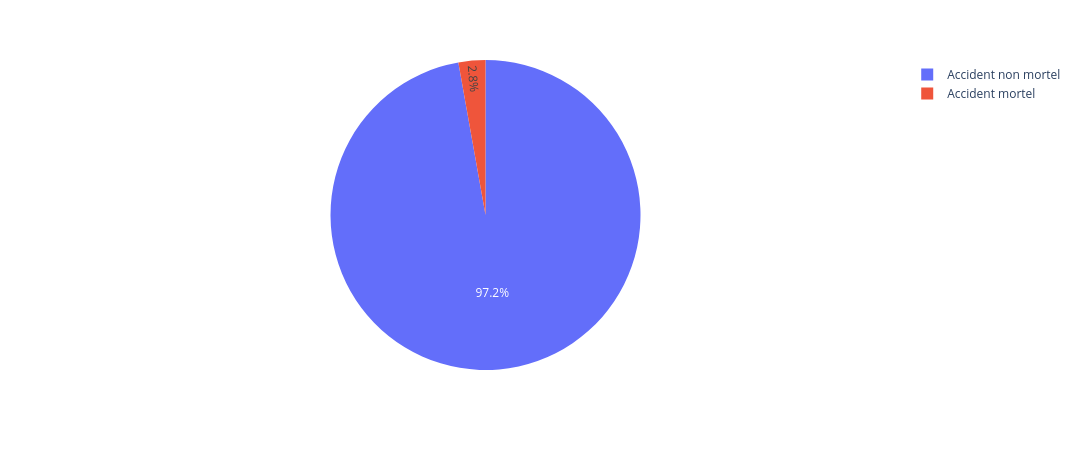
\includegraphics[width=12cm]{./img/grav1.png}
        \caption{Proportion d'accidents mortels}
    \end{figure}

    \section{Préparation des données}
    À partir des observations précédentes, nous avons supprimé les attributs moins intéressant pour l'apprentissage 
    et nous avons modifié certains attributs afin d'en extraire les informations intéressantes.
    \\
    Les attributs supprimés sont: \textit{voie}, \textit{v1}, \textit{v2}, \textit{pr}, \textit{pr1}, \textit{lartpc},
     \textit{larrout}, \textit{num\_veh}, \textit{occutc}, \textit{adr}, \textit{senc}, \textit{etatp}, \textit{actp}, 
     \textit{manv}, \textit{jour}, \textit{com}, \textit{hrmn}, \textit{motor}, \textit{place}, \textit{vosp}, \textit{locp}.
    \\\\
    Nous avons effectué les modifications suivantes:
    \begin{itemize}
        \item Création d'un attribut \textit{mortal} qui vaut 1 si le véhicule est impliqué dans un accident mortel, 0 sinon.
        \item À partir de l'attribut \textit{sexe} nous avons créé un attribut \textit{sexe\_conducteur} qui garde seulement 
                le sexe du conducteur du véhicule.
        \item Création d'un attribut \textit{piéton} qui vaut 1 si un piéton est impliqué dans l'accident, sinon 0.
        \item Nous avons utilisé l'année de naissance et l'année de l'accident pour récupérer l'âge du conducteur.
        \item L'attribut \textit{vma} a été découpé en 4 catégories de vitesse.
        \item Pour les attributs \textit{catv} et \textit{vatr} nous avons gardé les valeurs le plus représentées dans la base de données.
    \end{itemize}
    \vspace{0.5cm}
    Nous avons également reduit les valeurs de certains attributs. Par exemple pour des attributs 
    avec des valeurs telles que \textit{Non-renseigné}, \textit{Autre} \dots \, Nous avons regroupé 
    ces valeurs en une seule valeur. L'objectif était ici de simplifier en réduisant les catégories 
    mais également d'améliorer les performances de notre modèle.

    \section{Analyse des données}
    Une fois nos données préparées, nous avons pu les visualiser. Nous allons montrer dans les 
    deux prochaines parties les observations intéressantes que nous avons pu faire lors de 
    l'analyse de notre dataset.

    \subsection{Analyse univarié des données}
    \subsubsection{Les accidents mortels}
    Une donnée intéressante à observer est la proportion de véhicules impliqués dans un accident 
    mortel. C'est en effet la valeur que nous voulons prédire.

    \begin{figure}[ht]
        \centering
        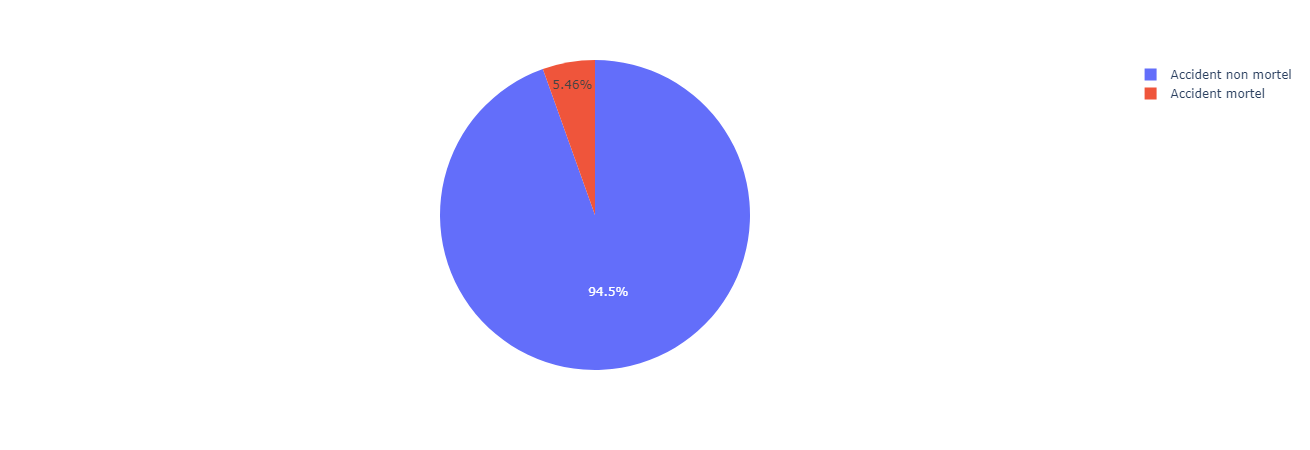
\includegraphics[width=10cm]{./img/grav2.png}
        \caption{Proportion des véhicules impliqués dans un accident mortel}
        \label{fig:fig_acc_mortel}
    \end{figure}

    Nous pouvons remarquer sur la figure \ref{fig:fig_acc_mortel} que le fait de s'intéresser 
    aux véhcules impliqués dans un accident mortel et non plus aux personnes victimes permet 
    de doubler le pourcentage. Même si cette proportion reste faible, cela va nous permettre 
    d'avoir plus de données dans la catégorie mortel lors de l'apprentissage et par conséquent 
    d'avoir un meilleur modèle.

    \subsubsection{Les piétons}
    Nous nous sommes ensuite intéressé aux accidents dans lesquels un piéton est impliqué. 
    La figure \ref{fig:fig_acc_pieton} nous montre qu'un peu moins de 10\% des accidents impliquent 
    un piéton.

    \begin{figure}[ht]
        \centering
        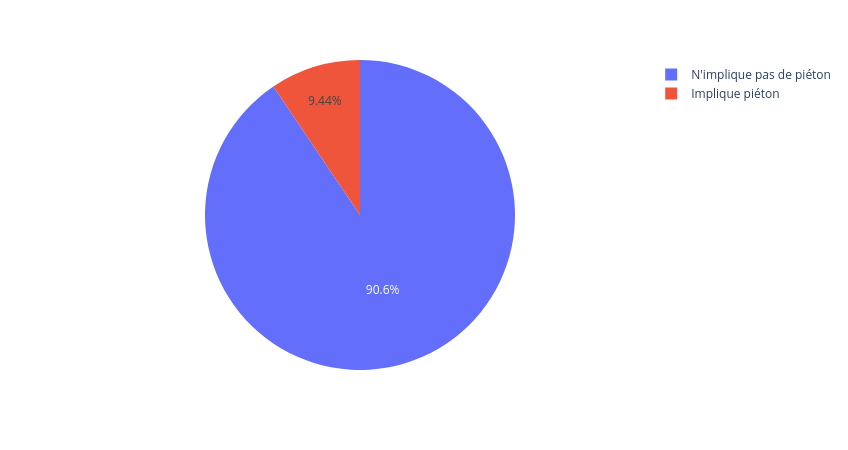
\includegraphics[width=10cm]{./img/pieton.png}
        \caption{Proportion des accidents avec piéton}
        \label{fig:fig_acc_pieton}
    \end{figure}

    \subsubsection{L'âge}
    Nous pouvons visualiser l'âge des conducteurs via une boîte à moustache. La figure \ref{fig:fig_age} nous 
    montre la répartition de l'âge des conducteurs. Lors du prétraitement des données, les valeurs aberrantes 
    ont été enlevée. On retrouve donc logiquement des âges contenus entre 0 et 100 ans. L'âge médian des 
    conducteurs est 33 ans avec le premier quatile à 21 et le troisième quatile à 49 ans. Même si on peut 
    imaginer que des valeurs sont fausse (il y a des conducteurs de moins de 16 ans), les valeurs sont tout de 
    même assez cohérentes par rapport à ce que l'on pourrait imaginer de la répartition de l'âge des conducteurs.

    \begin{figure}[ht]
        \centering
        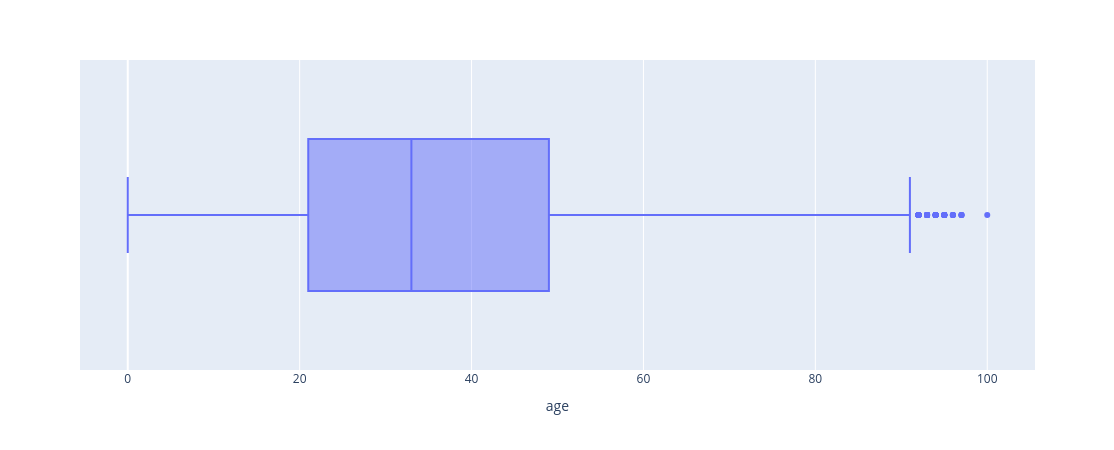
\includegraphics[width=12cm]{./img/age.png}
        \caption{Âge des conducteurs}
        \label{fig:fig_age}
    \end{figure}

    \subsubsection{Le genre des conducteurs}
    Le genre des conducteurs est assez intéressant à analyser. Sur la figure \ref{fig:fig_genre} nous pouvons 
    remarquer différence importante entre le nombre de femme au volant (indice 0) et le nombre d'hommes au volant 
    (indice 1). Cette différence pourrait être une source de biais pour notre modèle. En effet le fait qu'il y ait 
    beaucoup plus de données d'accident avec des hommes ne signifie pas qu'il y a plus de chance d'avoir un accident 
    si on est un homme. Cela signifie peut-être que la proportion d'homme au volant est plus élévée et donc qu'il 
    y a plus d'accident avec un homme au volant car il y a plus d'homme au volant. Le risque ici est que notre 
    modèle associe une homme à un accident mortel car il y a beaucoup plus d'accidents mortels avec un homme au 
    volant.

    \begin{figure}[ht]
        \centering
        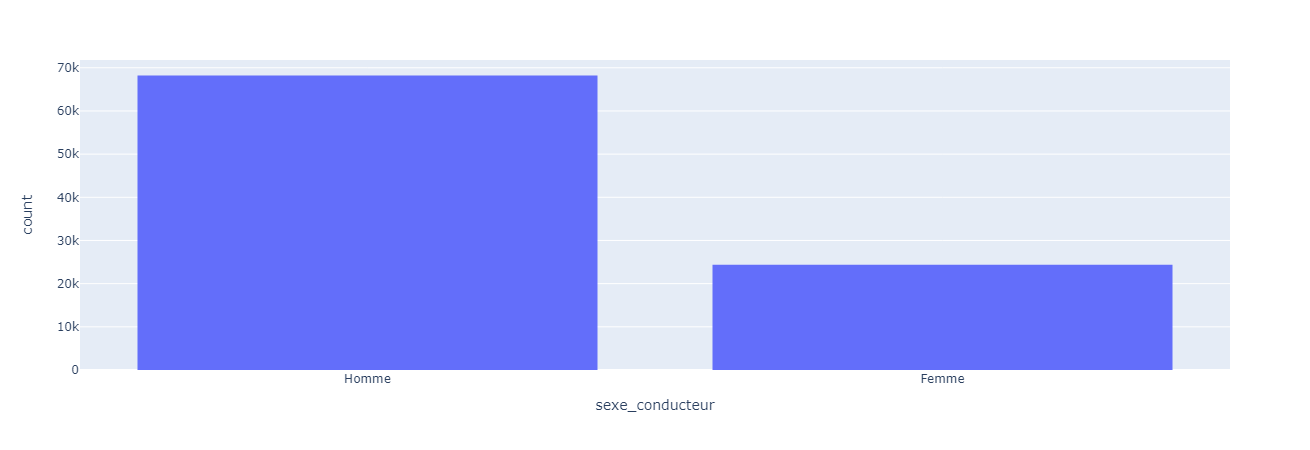
\includegraphics[width=12cm]{./img/sexe.png}
        \caption{Genre des conducteurs}
        \label{fig:fig_genre}
    \end{figure}

    \subsubsection{Le type de collision}
    La figure \ref{fig:fig_col} montre la répartition des différents types de collisions dans notre dataset. On peut 
    remarquer que tous les types de collisions sont plutôt bien représentés dans notre dataset. C'est un attribut qui 
    pourra être assez intéressant pour l'apprentissage.

    \begin{figure}[ht]
        \centering
        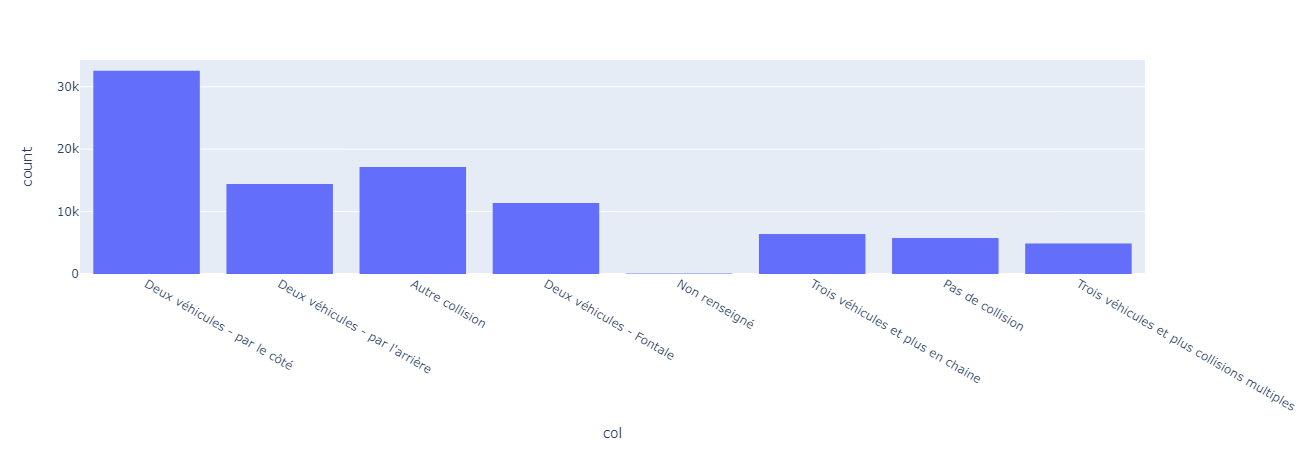
\includegraphics[width=12cm]{./img/col.png}
        \caption{Les types de collision}
        \label{fig:fig_col}
    \end{figure}

    \subsection{Analyse bivariée des données}
    Nous allons dans cette partie donner quelques exemples intéressant obtenus lors de l'analyse bivariée. On 
    peut retrouver l'ensemble des graphiques observés dans le fichier \texttt{main.ipynb}.

    \subsubsection{Le genre du conducteur}
    Un attribut qu'il est intéressant d'analyser est le genre du conducteur. En effet il peut être source de biais 
    s'il y a un déséquilibre entre homme et femme.
    On retrouve globalement la même proportion dans la corrélation que l'on soit homme ou femme. Les hommes étant 
    beaucoup plus représentés dans le dataset, la proportion d'hommes est logiquement plus élevée. On peut cependant 
    faire quelques remarques. 
    
    La figure \ref{fig:fig_sexe_bivar1} nous montre une proportion de femme moins élevée quand \textit{obsm} vaut 
    6. La proportion de femmes est deux fois plus élevée quand \textit{obsm} vaut 1. Ceci pourrait biaiser notre 
    modèle.
    
    Sur la figure \ref{fig:fig_sexe_bivar2}, on remarque également une proportion différente de femmes 
    en fonction du type de véhicule. On pourrait expliquer cela par le fait que certains véhicules sont 
    dans la réalité plus utilisés par les hommes, par exemple pourrait imaginer qu'il y a plus d'hommes qui 
    conduisent des motos. Il faudra être vigilant car cela peut être source de biais. Il se peut que notre 
    modèle associe une moto à un homme. Et que dans le cas d'une femme sur une moto le résultat soit soit 
    forcément un accident mortel, soit forcément un accident non mortel.

    \begin{figure}[h]
        \begin{subfigure}{6cm}
            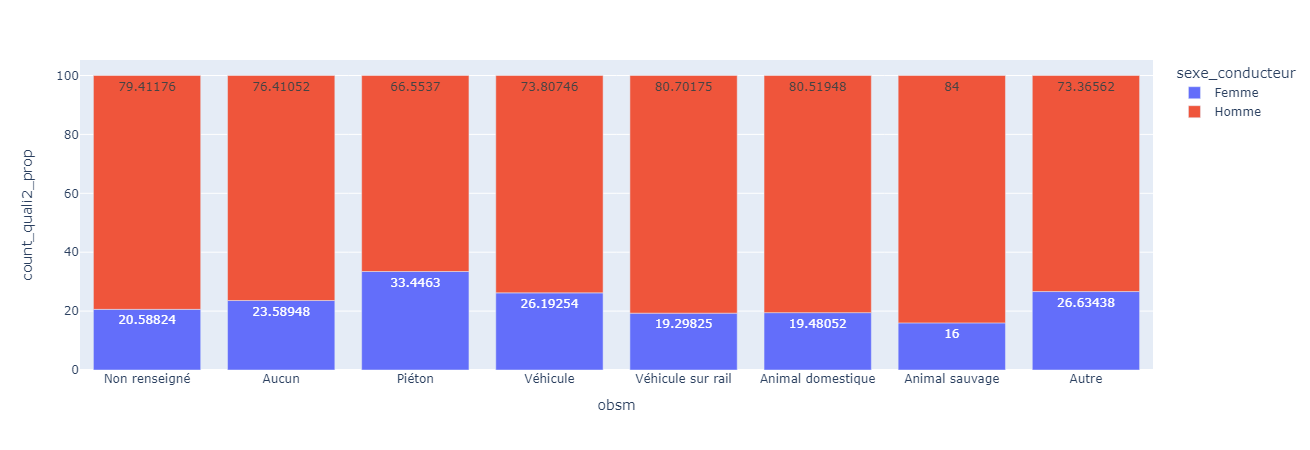
\includegraphics[width=6cm]{./img/bivar_sexe.png}
            \caption{Variation de la proportion de femme en fonction de la présence d'un obstacle dans l'accident}
            \label{fig:fig_sexe_bivar1}
        \end{subfigure}
        \begin{subfigure}{6cm}
            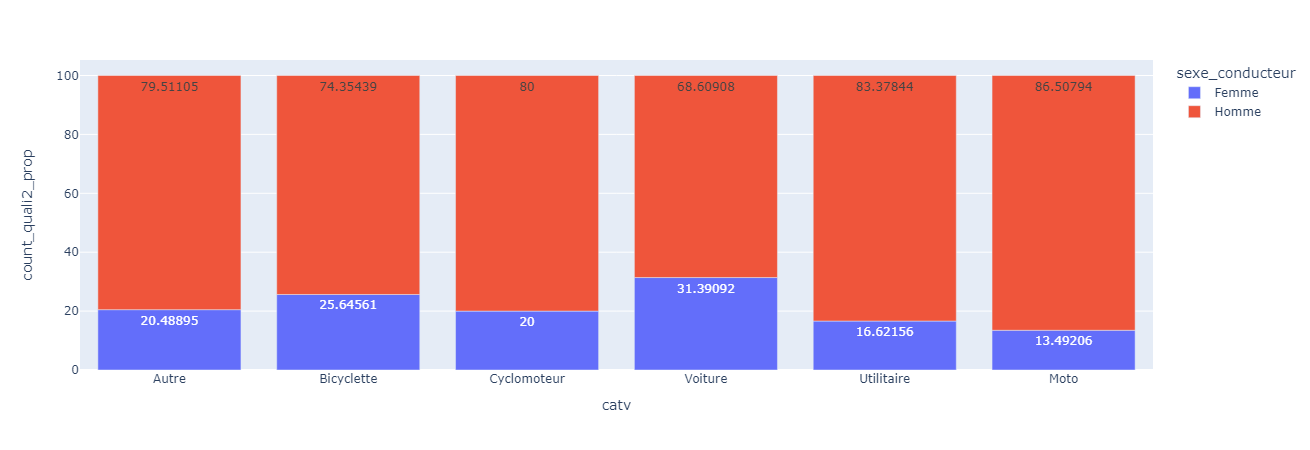
\includegraphics[width=6cm]{./img/bivar_sexe2.png}
        \caption{Variation de la proportion de femme en fonction de la présence d'un obstacle dans l'accident}
        \label{fig:fig_sexe_bivar2}
        \end{subfigure}
    \end{figure}

    \section{Apprentissage}
    
    \subsection{Split}
    Séparer nos données en deux sets demandait de tenir compte d'une spécéificité. Nous nous plaçons du point de vue d'un véhicule. 
    Mais c'est bien souvent plusieurs véhiécules qui sont impliqués dans un accident. Il nous a donc fallut adapter le split pour que 
    les véhicule d'un même accident soit dans le même set. 
    
    Par ailleurs, nous avons pu constater que ne pas adopter cette approche, provoquait un overfit lors du test. Typiquement, un trop 
    grand nombre de mort était trouvés avec succès.

    \subsection{One Hot Encoding}
    La base de donnée nous fournit pour la plus part des attributs des données qui sont convertibles en entiers. 
    Par exemple une catégorie de véhicule (\textit{catv}) est dénomée par un chiffre. L'attribut cependant reste catégoriel. Dans les faits, 
    Le seul attribut quantitatif qu'il nous reste est l'âge du conducteur. 
    Le reste est soit binaire, soit qualitatif. 
    
    Tous les attributs qualitatifs ont donc été transformés en OneHot. Au départ nous souhaitions optimiser le nombre de colonnes en 
    faisant les one hot par nous même. Typiquement, preonons surf (l'état de la surface de la route). Il est inutile de créer une colonne 
    Non-renseigné, Autre ou normale. Nous ne sommes intéressés que par les états spécifiques de la route. 

    Cet approche cependant était source d'ennuis puisqu'elle empêchait la réalisation de l'audit. Nous avons donc utilisés la méthode 
    standard pour nos oneHot. 

    \subsection{Random Tree Classifier}
    Une fois les données prêtes, nous avons utilisés le classifieur d'arbres aléatoires pour obtenir un modèle. C'est le premier que nous 
    avons utilisé. Pour ce qui est des résultats, l'accuracy score est de \textit{1} pour l'entrainement et de \textit{0.9014} pour le teste.
    
    Pour ce qui est de la matrice de confusion, on remarque que \textit{27687} véhcules ont été classés à raison en tant que accidents non létaux.
    Tandis que \textit{291} accidents mortels ont été trouvés. Toutefois \textit{1413} accidents mortel ont été resecés à tord comme étant 
    non létaux et \textit{1648} véhicule ont subit le sort inverse. 

    En résumé, on remaque que le modèle réussit très bien à classifier les accidents qui n'ont pas conduit à la mort de quelqu'un. Cemendant,
    il lui apparaît bien plus difficile de trouver les véhicules impliqués accidents qui sont mortels. On peut attribuer ceci au fait que
    ces accidents létaux ne représentent que \textit{5.38\%} des accidents rétertoriés dans la base.
    
    \subsection{GaussianNB}


    \section{Audit du modèle}

    \subsection{Génération des contrefactuels avec Dice}
    Dice nous a permis d'établir quels attributs influent sur la prédiction de notre modèle. Les résultats sont 
    cependant assez variants d'une exécution à l'autre. On peut tout de même retrouver lesquels sont fréquemment impliqués 
    dans le changement des exemples contrefactuels.
    Parmi eux on peut noter que \textit{âge} est souvent représenté. Le taux d'accidents (notamment mortels) étant plus 
    élevé chez les jeunes et les personnes âgées, cela paraît assez cohérent. L'attribut \textit{obsm} est également 
    souvent représenté dans les exemples contrefactuels.
    On a pu remarquer que l'attribut \textit{col} est peu représenté dans les résultats contrairement à l'hypothèse que 
    nous avions pu faire lors de l'analyse.
    
    Enfin les attributs \textit{dep} et \textit{sexe\_conducteur} sont également représentés. Ils pourraient être sources de biais, notamment 
    l'attribut \textit{dep}, le modèle pourrait associer un département à une prédiction d'accident mortel.



\end{document}